\chapter{Összefoglalás, konklúzió}

\todo[inline]{Bevezetendő intézkedések hatásának elemzése.}
\begin{wrapfigure}{R}{0.5\textwidth}
    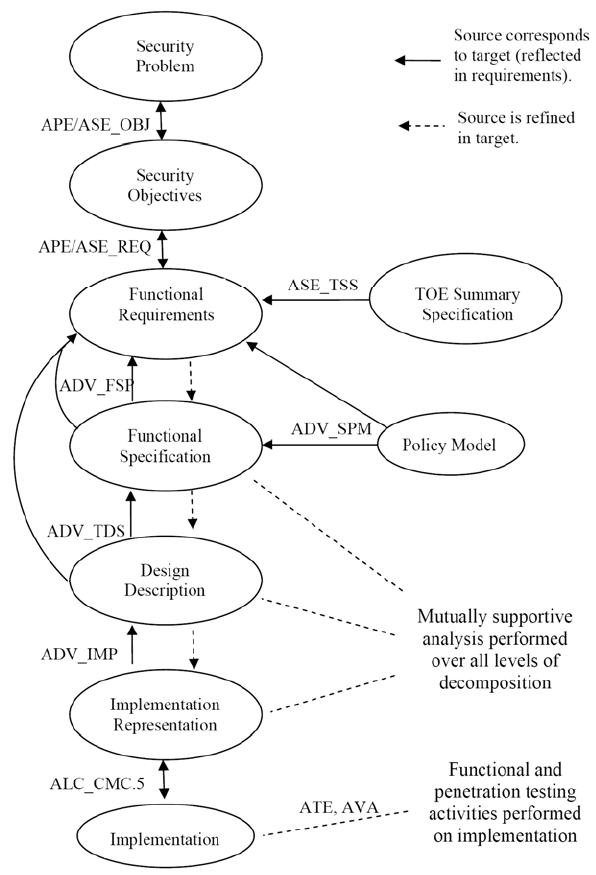
\includegraphics[width=0.45\textwidth, keepaspectratio]{figures/layers.png}
\end{wrapfigure}
\section{Értékelés}

Összességében úgy gondolom, hogy az érintett követelmények, és az azokra adott javaslatok bevezetése
mind a termékfejlesztés hatékonyságát, mind a biztosított minőséget, mind a termék biztonságát
növelte.


Tapasztalataim szerint azáltal, hogy a Common Criteria is rávilágít egyes anomáliákra, indokoltabbá
válhat ezeknek az anomáliáknak a felszámolása, az esetleges \emph{workaround}-ok kevésbé
tekinthetőek elfogadhatónak. Ez a pszichológiai hatás számomra váratlan volt, de mindenképpen
pozitívumként tekintek rá.

\section{Továbbfejlesztési lehetőségek}
Tekintve, hogy a szakdolgozat a Common Criteria követelményeinek csupán egy kis, valódi részhalmazát
dolgozta fel, például az egyik leglényegesebb, és időigényesebb, (biztonsági) funkcionalitással
foglalkozó osztályai nem kerültek tárgyalásra, így nem került említésre a Common Criteria egyik
lényeges funkciója, amely segít azt belátni, hogy az alacsonyabb szintű implementáció megoldást
nyújt a magas szinten lévő biztonsági problémára.
Úgy gondolom, hogy a szakdolgozatban elkezdett elemzés könnyedén folytatható a további osztályok
lefedésével, és a modernizálás utáni (amikor már a fejlesztők megszokták és elfogadták
a változtatásokat) tapasztalatok összegyűjtésével.
